\documentclass[14pt,t,aspectratio=169]{beamer}
\usepackage{fontspec}
\usepackage{color}
\usepackage{minted}
\usepackage{array}
\usepackage{emoji}
\usepackage{svg}

%% These fonts are non-free.
%% Comment out the lines if you don't have them.
\setmainfont{Equity Text A}
\setsansfont{Concourse T3}
\setmonofont{Triplicate T4}

\definecolor{bgcolor}{RGB}{255,240,240}
\definecolor{red}{RGB}{224,35,35}
\setbeamercolor{background canvas}{bg=bgcolor}
\setbeamercolor{normal text}{fg=black}
\setbeamercolor{titlelike}{fg=black}
\setbeamercolor{itemize item}{fg=red}
\setbeamercolor{enumerate item}{fg=red}
\setbeamertemplate{itemize items}[circle]
\setbeamertemplate{navigation symbols}{}
\usemintedstyle{monokai}
\newminted[lispcode]{common-lisp}{fontsize=\footnotesize}
\newminted[smalllispcode]{common-lisp}{fontsize=\scriptsize}
\def\code#1{{\color{codecolor}\texttt{#1}}}
\renewcommand{\theFancyVerbLine}{\color{darkgray}\large \oldstylenums{\arabic{FancyVerbLine}}}

\usebackgroundtemplate{
\includegraphics[width=\paperwidth,height=\paperheight]{background}}
\begin{document}
{\usebackgroundtemplate{
\includegraphics[width=\paperwidth,height=\paperheight]{firstpage}}
  \begin{frame}
    \color{white}
    \vspace{3cm}
    {\hspace{1.4cm} \LARGE Porting SBCL to the Nintendo Switch} \\
    \vspace{1cm}
    {\hspace{1.6cm} Yukari Hafner, Charles Zhang} \\
    \vspace{0.2cm}
    {\hspace{2.1cm}\texttt https://shirakumo.org}
  \end{frame}}

\begin{frame}
  \frametitle{The Device}
  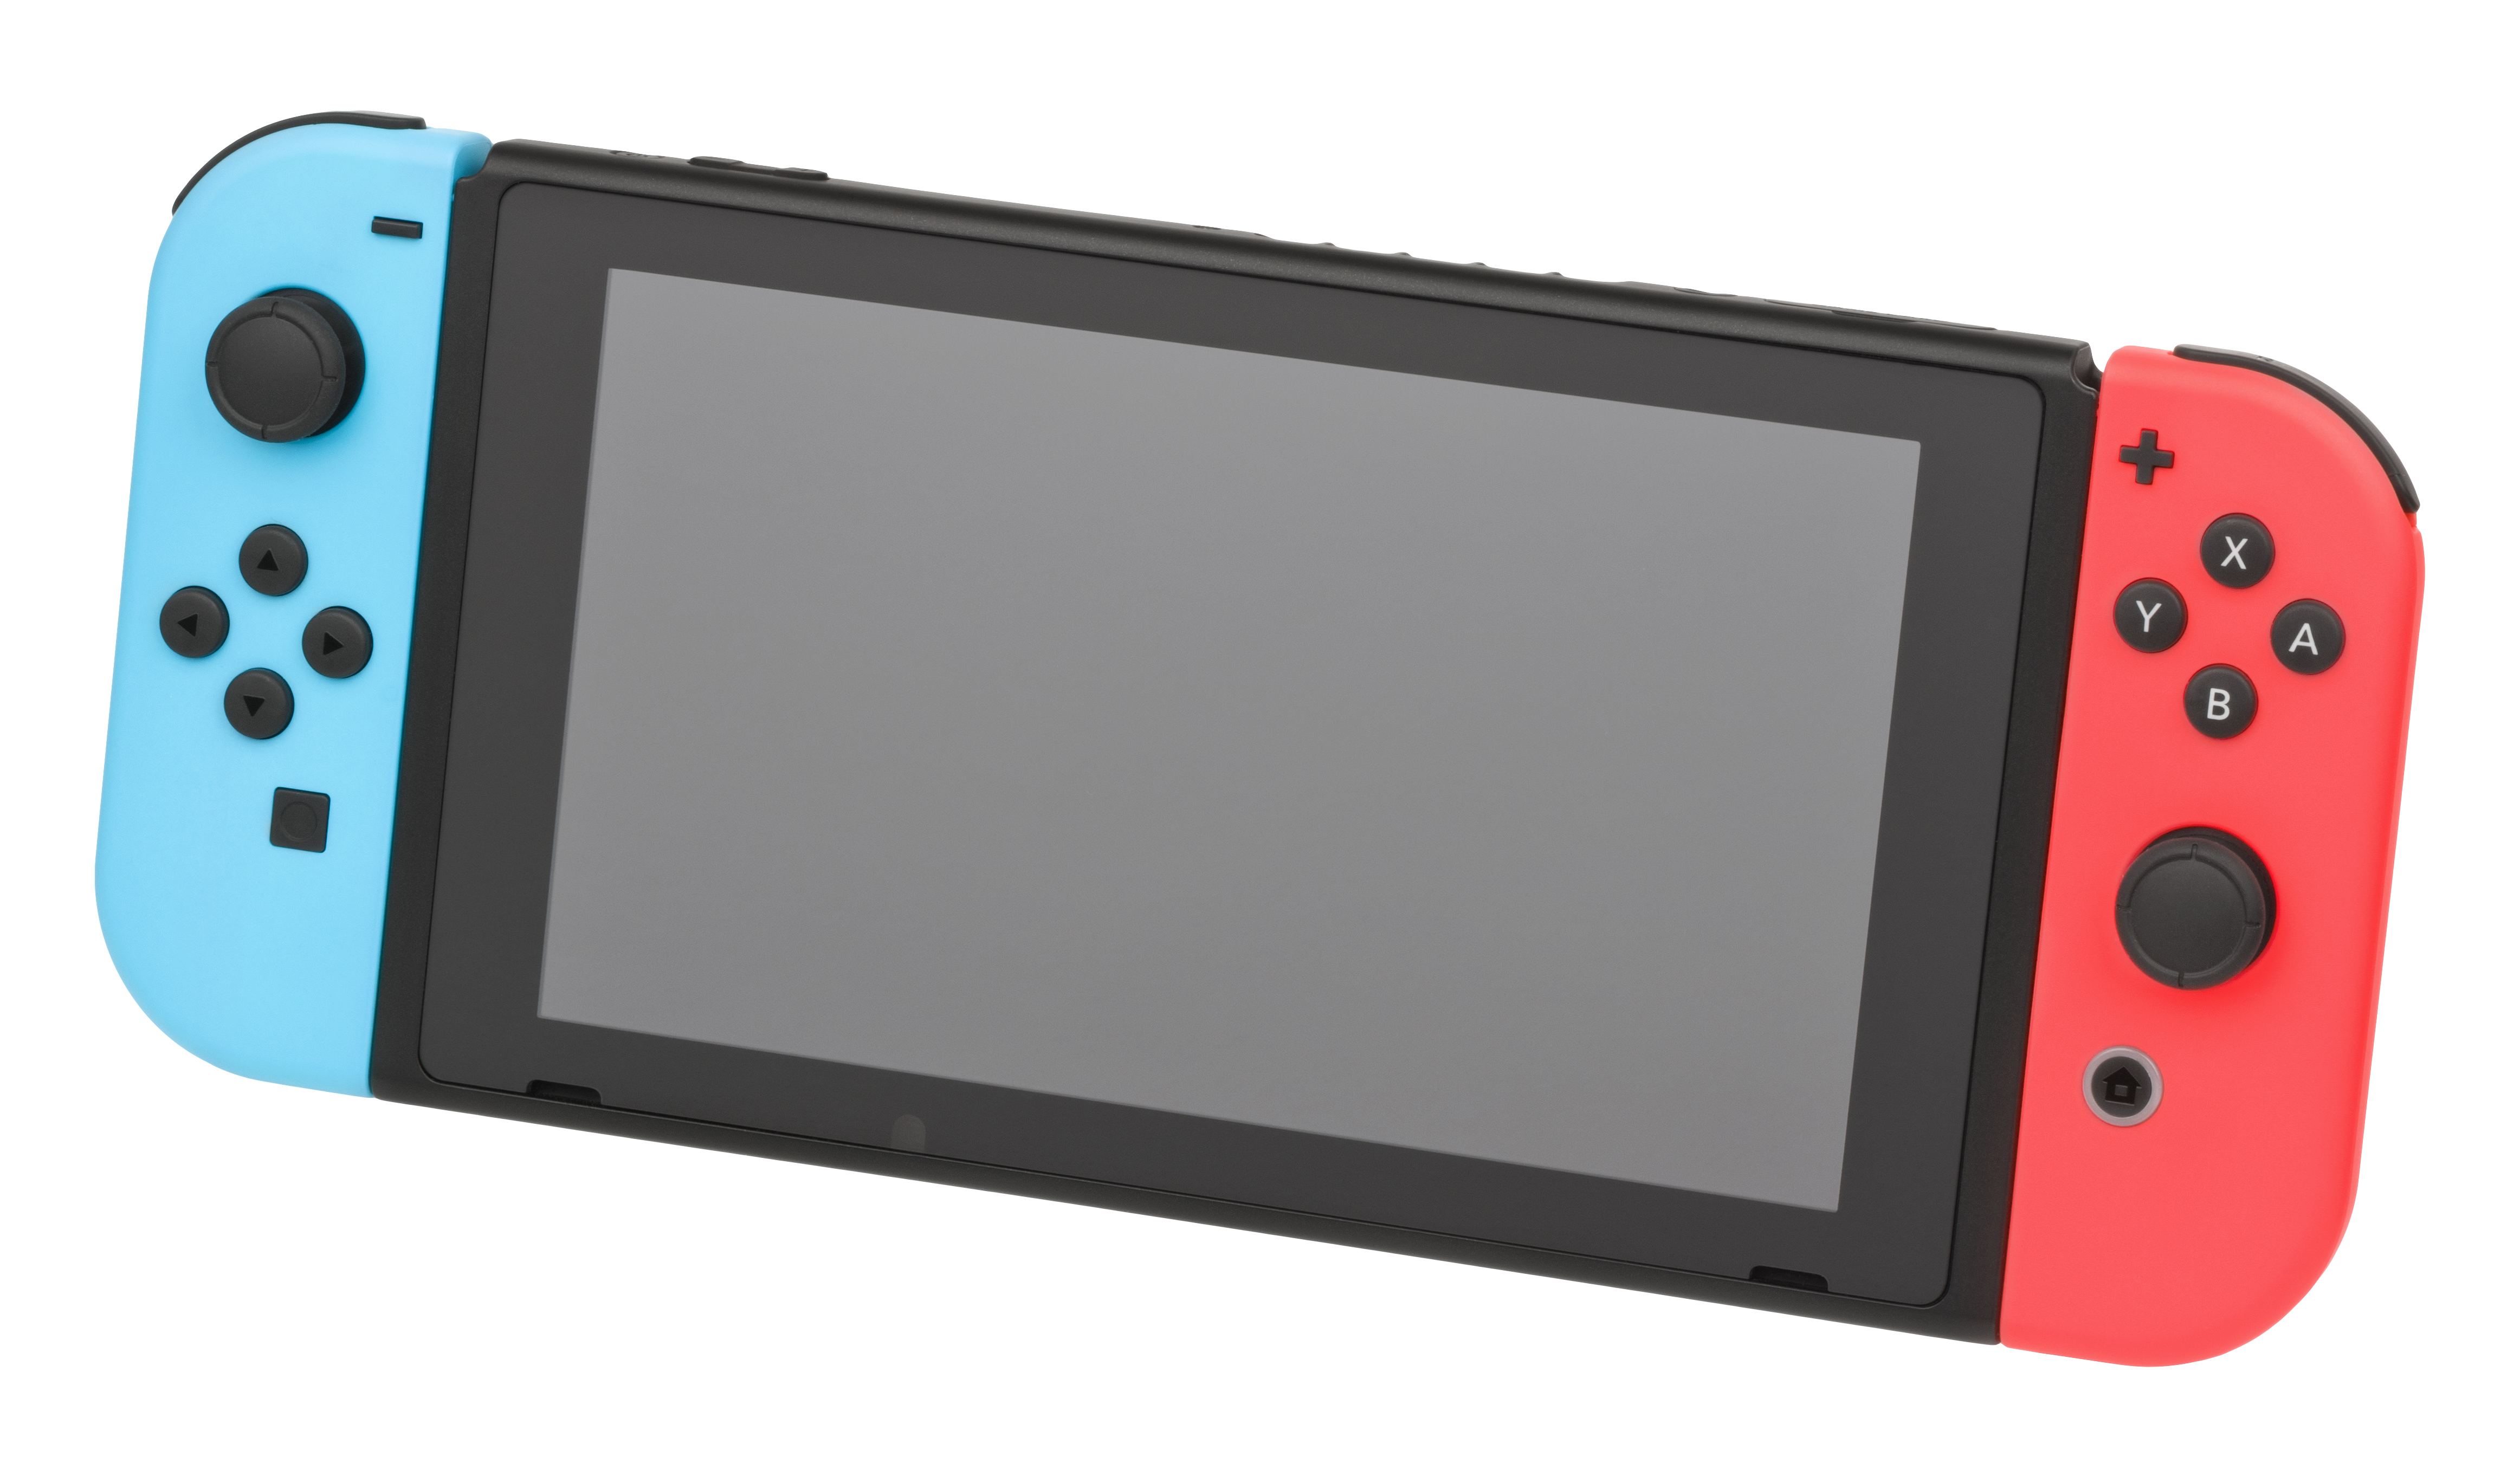
\includegraphics[height=5cm]{switch}
  \begin{itemize}
  \item CPU: ARM 4 Cortex-A57 64-bit
  \item OS: ``Horizon OS'', proprietary micro-kernel
  \item SDK: C++, proprietary version of Clang
  \end{itemize}
\end{frame}

\begin{frame}
  \frametitle{Immediate Challenges}
  \begin{itemize}
  \item Everything is proprietary and under NDA \\
    \Rightarrow{} Scarce public information
  \item The OS is not BSD or even fully POSIX \\
    \Rightarrow{} Need new OS abstractions
  \item There are no inter-thread signals \\
    \Rightarrow{} Can't use usual GC tricks
  \item We are not allowed to create executable pages \\
    \Rightarrow{} No compilation at runtime
  \end{itemize}
\end{frame}

\begin{frame}
  \frametitle{Basic Ideas}
  \begin{itemize}
    \color{lightgray}
  \item Everything is proprietary and under NDA \\
    \textcolor{red}{\Rightarrow} \textcolor{black}{Only publicise our own interfaces}
  \item The OS is not BSD or even fully POSIX \\
    \textcolor{red}{\Rightarrow} \textcolor{black}{Write C(++) shim libraries for access}
  \item There are no inter-thread signals \\
    \textcolor{red}{\Rightarrow} \textcolor{black}{Use safepoints}
  \item We are not allowed to create executable pages \\
    \textcolor{red}{\Rightarrow} \textcolor{black}{Compile everything on linux
      and shrinkwrap}
  \item The OS enforces strict Address Space Layout Randomization (ASLR) \\
    \textcolor{red}{\Rightarrow} \textcolor{black}{Make all code and data fully
      relocatable and position independent}
  \end{itemize}
\end{frame}

\begin{frame}
  \frametitle{History of the Project}
  \begin{itemize}
  \item Initial discussion on \#sbcl and at ELS 2022 about porting SBCL
    to Nintendo Switch \\
  \item Decided to seriously pursue project at ELS 2023 \\
    \Rightarrow{} Sketched out project plan in the airport afterwards
  \item Most of the initial work and design problems solved in the
    following months \\
  \item Debugging GC issues and improving debugging experience in
    2024 \\
  \item Game engine examples stabilized, Kandria running in early 2025 \\
  \end{itemize}
\end{frame}

\begin{frame}
  \frametitle{A Standard SBCL Build}
  \begin{itemize}
  \item build-config \\
    \Rightarrow{} Gather system info
  \item make-host-1 \\
    \Rightarrow{} Emit C headers and support files
  \item make-target-1 \\
    \Rightarrow{} Compile the C runtime on the target
  \item make-host-2 \\
    \Rightarrow{} Cross-compile the compiler on the host
  \item make-target-2 \\
    \Rightarrow{} Use the compiler from the host to\\ incrementally compile the rest on the target
  \end{itemize}
\end{frame}

\begin{frame}
  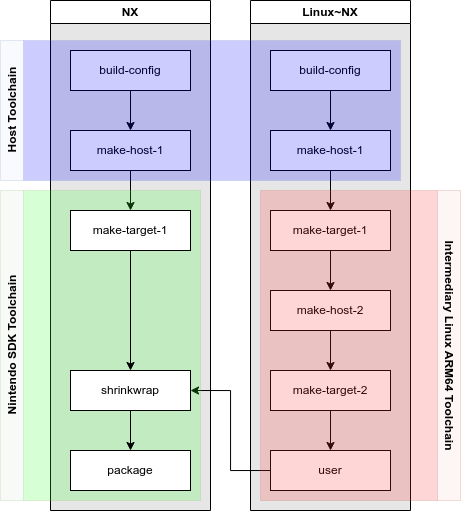
\includegraphics[height=8.5cm]{build.png}
\end{frame}

\begin{frame}
  \frametitle{Relocation}
  \begin{itemize}
  \item Lisp objects are full of absolute pointers to other objects
  \item Lisp objects live in Lisp spaces mapped at fixed addresses
  \item Saving an image dumps Lisp spaces to disk verbatim
  \item Reloading an image is fast; just \texttt{mmap} the on-disk
    spaces into the process.
  \item \Rightarrow{} Problem for NX: enforced ASLR means no means to map spaces
    to desired addresses
  \end{itemize}
\end{frame}

\begin{frame}
  \frametitle{Relocation (cont.)}
  \begin{itemize}
    \item Solution: Relocate all Lisp spaces on start up
    \item \Rightarrow{} Problem for NX: Code generation hardwires some primitive
      object addresses.
    \item Solution: Change codegen to be position independent.
    \item Code objects in SBCL also contain Lisp pointers (constants)
    \item \Rightarrow{} Problem for NX: Relocation and moving GC needs to fix up
      these constants, but code objects are not writable
    \item Solution: Segregate code instructions and data in code
      objects into different ELF sections offline, rewrite code
      instructions to reference r/w section
  \end{itemize}
\end{frame}

\begin{frame}
  \frametitle{Relocation example}
  XXX why doesn't this work?
%   \begin{listing}
%     \begin{minted}[fontsize=\small]{lisp}
% (defun f ()
%   (cons '(42 . 1958) 'els2025))

%      \end{minted}
%   \caption{A Lisp function referencing the constants \code{'(42 . 1958)} and \code{'ELS2025}.}
%   \label{lst:function}
%   \end{listing}
\end{frame}

\begin{frame}
  \frametitle{Relocation example (cont.)}
  \begin{figure}[h]
    \centering
    \includesvg[width=\linewidth]{Code object before shrinkwrapping.drawio.svg}
    \caption{Representation of the compiled code object (in boldface)
      for the function \protect\texttt{\#'f} in memory, along with the
      cons and symbol objects it references.}
    \label{fig:before-shrinkwrap}
  \end{figure}
\end{frame}

\begin{frame}
  \frametitle{Relocation example (cont.)}
  \begin{figure}[h]
    \centering
    \includesvg[width=\linewidth]{Code objects in memory after shrinkwrapping.drawio.svg}
    \caption{Representation of the same code object and the cons and
      symbol objects it references after code/data segregation and the
      rest of the shrinkwrapping process.}
    \label{fig:after-shrinkwrap}
  \end{figure}
\end{frame}

\begin{frame}
  \frametitle{Garbage Collection}
  \begin{itemize}
  \item Garbage collection on SBCL on non-Windows platforms uses POSIX
    signals to stop-the-world.
  \item \Rightarrow{} Problem for NX: No POSIX signals.
  \item Solution: Use safepoints (implemented already on Windows)
  \item BUT: The safepoint mechanism still uses virtual memory
    hardware exceptions to stop the current thread
  \item \Rightarrow{} Problem for NX: No ability to handle operating system
    exceptions
  \item Solution: Change safepoint codegen to poll state flags
    explicitly
  \end{itemize}
\end{frame}

\begin{frame}
  \frametitle{Misc Issues}
  \begin{itemize}
  \item SBCL uses hardware exceptions to signal some common conditions
  \item \Rightarrow{} Solution: Change to full calls to \texttt{ERROR} and \texttt{SIGNAL}
  \item CLOS requires runtime compilation for dispatch JIT
  \item \Rightarrow{} Solution: Use an interpreter where absolutely necessary
  \item The existing shrinkwrap tool is not GC-safe for precise GC
    platforms like ARM64, random crashes with large cores
  \item  \Rightarrow{} Solution: Complicate the build process even more by using
    a separate SBCL with memory spaces mapped away from the offline
    core's spaces to shrinkwrap
  \end{itemize}
\end{frame}

\begin{frame}[c]{ }
  \centering
  {\Huge Live Demo}
\end{frame}

\begin{frame}
  \frametitle{Further Work}
  \begin{itemize}
  \item Optimising CLOS dispatch ahead of time \\
    \Rightarrow{} Christophe? \emoji{pleading-face}
  \item Optimising Trial and Kandria \\
    \Rightarrow{} Lots of profiling work that can be done on PC
  \item Porting to the Nintendo Switch 2 \\
    \Rightarrow{} As soon as plebians like us get access from almighty \\\quad Nintendo
  \end{itemize}
\end{frame}

{\usebackgroundtemplate{
\includegraphics[width=\paperwidth,height=\paperheight]{firstpage}}
  \begin{frame}[c]{ }
    \centering\color{white}
    \vspace{2cm}
    {\LARGE Thank you!} \\
    \vspace{0.2cm}
    Consider supporting our work: \\
    
\includegraphics[width=3cm]{patreon} \\
    {\texttt https://patreon.com/shinmera}
  \end{frame}}
\end{document}

%%% Local Variables:
%%% mode: latex
%%% TeX-master: t
%%% TeX-engine: luatex
%%% TeX-command-extra-options: "-shell-escape"
%%% End:
